% CREATED BY DAVID FRISK, 2016
\chapter{Results}
\section{Experiment 1: Baseline Evaluation \& Blindfolding}
Fig.~\ref{fig:training_metrics} shows metrics for each batch during training. Fig.~\ref{fig:baseline_metrics} shows metrics averaged for each epoch during the baseline evaluation. Fig.~\ref{fig:blindfolded_metrics} shows metrics averaged for each epoch during blindfolded evaluation. It's clear in these graphs that the evaluation results are more stable when the model is given images. As can be seen in Figures~\ref{fig:baseline_loss} \& ~\ref{fig:blindfolded_loss}, the model begins to overfit to the training data around epoch 10. \newline
Table~\ref{tab:best_baseline} shows the checkpoints with lowest loss, highest accuracy, and lowest mean rank during the evaluation of the baseline, with the metric that was "best" during that checkpoint in bold. Table~\ref{tab:best_blindfolded} shows the same for blindfolded evaluation. Comparing their best, the blindfolded model has 4.7\% worse loss than the baseline, 0.212 higher loss, and 0.149 higher mean rank. \newline
One question here is whether the blank inputs to the model are actively confusing it--in training it is always given an image, so this black input is a completely new case. This could also explain the differences to a previous student's course project, in which they found equivalent performance to baseline when the agent was given a random image from the dataset. One challenge here is that scenes are used for multiple questions, so this leaves open the possibility that the item being asked about is actually present in the room. Even using scenes not included in the dataset would be difficult to control, since if you ask the agent 'what color is the bookshelf?', you would then need to confirm that no bookshelves are present in the random image. \newline
\begin{figure}[ht!]
	\centering
	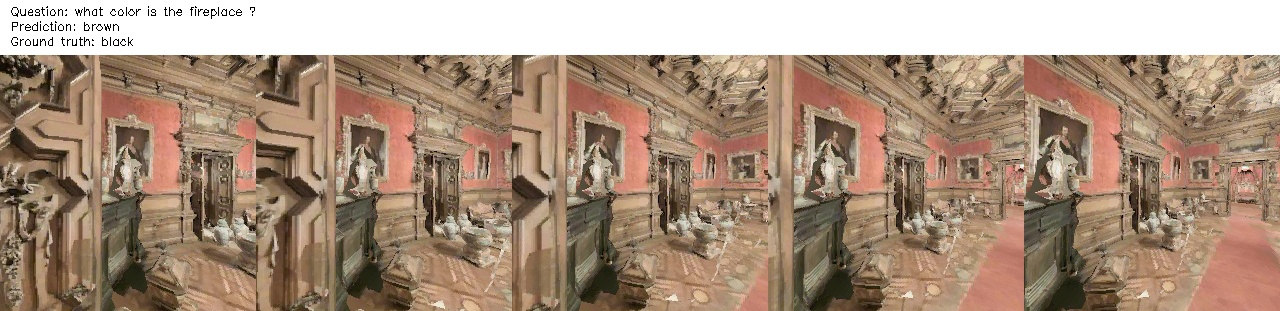
\includegraphics[width=\textwidth]{/home/yasmeen/Desktop/thesisproj/thesis/figure/results/baseline_and_blindfolding/images/ckpt_23_781_image.jpg}
	\caption{Example VQA Result}
	\label{fig:example_vqa_result}
\end{figure}
	

\begin{figure}[ht!]
	\centering
	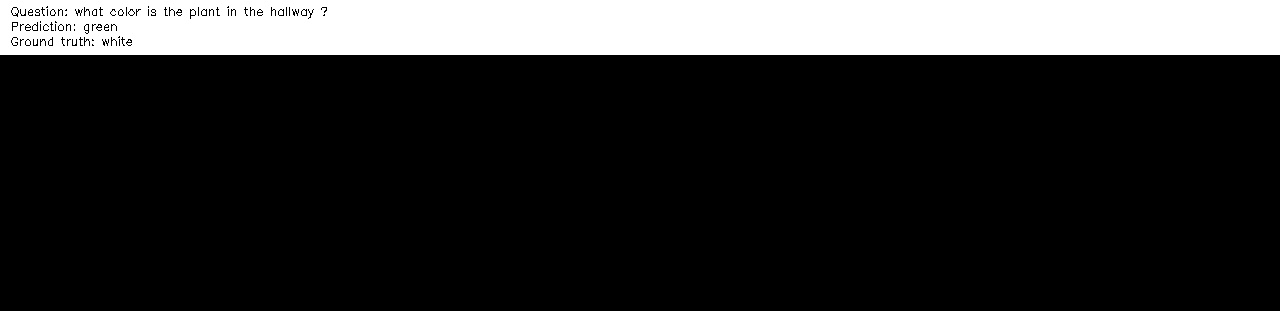
\includegraphics[width=\textwidth]{/home/yasmeen/Desktop/thesisproj/thesis/figure/results/baseline_and_blindfolding/blindfolded/ckpt_23_1250_image.jpg}
	\caption{Example Blindfolded Result}
	\label{fig:example_blindfolded_result}
\end{figure}

\begin{figure}[ht!]
     \centering
     \begin{subfigure}[b]{0.3\textwidth}
         \centering
         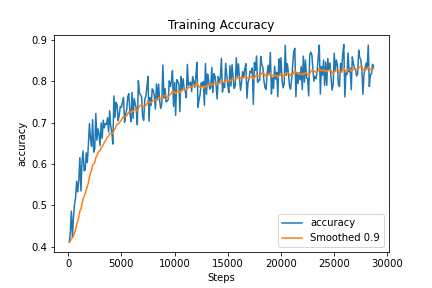
\includegraphics[width=\textwidth]{/home/yasmeen/Desktop/thesisproj/thesis/figure/results/baseline_and_blindfolding/training/accuracy.png}
         \caption{Training Accuracy}
         \label{fig:training_accuracy}
     \end{subfigure}
     \hfill
     \begin{subfigure}[b]{0.3\textwidth}
         \centering
         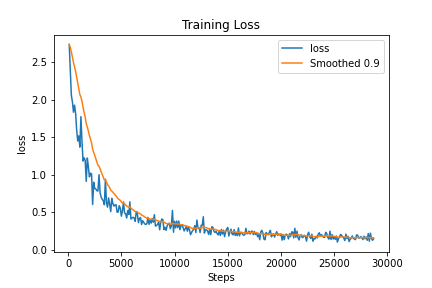
\includegraphics[width=\textwidth]{/home/yasmeen/Desktop/thesisproj/thesis/figure/results/baseline_and_blindfolding/training/loss.png}
         \caption{Training Loss}
         \label{fig:training_loss}
     \end{subfigure}
     \hfill
     \begin{subfigure}[b]{0.3\textwidth}
         \centering
         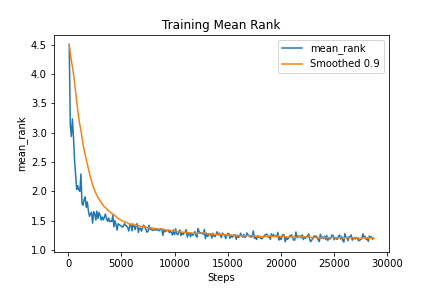
\includegraphics[width=\textwidth]{/home/yasmeen/Desktop/thesisproj/thesis/figure/results/baseline_and_blindfolding/training/mean_rank.png}
         \caption{Training Mean Rank}
         \label{fig:training_mean_rank}
     \end{subfigure}
     \caption{Training Metrics}
     \label{fig:training_metrics}
\end{figure}

\begin{figure}[ht!]
     \centering
     \begin{subfigure}[b]{0.3\textwidth}
         \centering
         \includegraphics[width=\textwidth]{/home/yasmeen/Desktop/thesisproj/thesis/figure/results/baseline_and_blindfolding/images/avg val accuracy.png}
         \caption{Baseline Validation Accuracy}
         \label{fig:baseline_accuracy}
     \end{subfigure}
     \hfill
     \begin{subfigure}[b]{0.3\textwidth}
         \centering
         \includegraphics[width=\textwidth]{/home/yasmeen/Desktop/thesisproj/thesis/figure/results/baseline_and_blindfolding/images/avg val loss.png}
         \caption{Baseline Validation Loss}
         \label{fig:baseline_loss}
     \end{subfigure}
     \hfill
     \begin{subfigure}[b]{0.3\textwidth}
         \centering
         \includegraphics[width=\textwidth]{/home/yasmeen/Desktop/thesisproj/thesis/figure/results/baseline_and_blindfolding/images/avg val mean rank.png}
         \caption{Baseline Validation Mean Rank}
         \label{fig:baseline_mean_rank}
     \end{subfigure}
     \caption{Baseline Validation Metrics}
     \label{fig:baseline_metrics}
\end{figure}


\begin{figure}[ht!]
     \centering
     \begin{subfigure}[b]{0.3\textwidth}
         \centering
         \includegraphics[width=\textwidth]{/home/yasmeen/Desktop/thesisproj/thesis/figure/results/baseline_and_blindfolding/blindfolded/avg val accuracy.png}
         \caption{Blindfolded Validation Accuracy}
         \label{fig:blindfolded_accuracy}
     \end{subfigure}
     \hfill
     \begin{subfigure}[b]{0.3\textwidth}
         \centering
         \includegraphics[width=\textwidth]{/home/yasmeen/Desktop/thesisproj/thesis/figure/results/baseline_and_blindfolding/blindfolded/avg val loss.png}
         \caption{Blindfolded Validation Loss}
         \label{fig:blindfolded_loss}
     \end{subfigure}
     \hfill
     \begin{subfigure}[b]{0.3\textwidth}
         \centering
         \includegraphics[width=\textwidth]{/home/yasmeen/Desktop/thesisproj/thesis/figure/results/baseline_and_blindfolding/blindfolded/avg val mean rank.png}
         \caption{Blindfolded Validation Mean Rank}
         \label{fig:blindfolded_mean_rank}
     \end{subfigure}
     \caption{Blindfolded Validation Metrics}
     \label{fig:blindfolded_metrics}
\end{figure}

\begin{table}[ht!]
\centering
\caption{"Best" Epochs During Baseline Evaluation}
\begin{tabular}{l | l | l | l}
Checkpoint & Loss & Accuracy & Mean Rank \\
\hline
8 & \textbf{2.204141} & 0.381122 & 4.341837 \\
15 & 2.404433 & \textbf{0.403061} & 4.138265 \\
23 & 2.691763 & 0.370408 & \textbf{4.110714}
\end{tabular}
\label{tab:best_baseline}
\end{table}

\begin{table}[ht!]
\centering
\caption{"Best" Epochs During Blindfolded Evaluation}
\begin{tabular}{l | l | l | l}
Checkpoint & Loss & Accuracy & Mean Rank \\
\hline
5 & \textbf{2.416477} & 0.246429 & 5.493877 \\
27 & 2.546098 & \textbf{0.355612} & 4.551021 \\
39 & 4.788071 & 0.307653 & \textbf{4.260204}
\end{tabular}
\label{tab:best_blindfolded}
\end{table}


\section{Experiment 2: Basic Semantic Categories}
In this experiment, the model was provided with semantic category information, as described in \ref{sec:exp_2}.
With the categories, the highest accuracy was 1.4\% higher than the baseline's highest accuracy, and the highest mean rank was 0.46 higher than the baseline's highest. \newline

\begin{figure}[ht!]
     \centering
     \begin{subfigure}[b]{0.3\textwidth}
         \centering
         \includegraphics[width=\textwidth]{/home/yasmeen/Desktop/thesisproj/thesis/figure/results/semantic_categories/eval/avg val accuracy.png}
         \caption{Validation Accuracy}
         \label{fig:category_accuracy}
     \end{subfigure}
     \hfill
     \begin{subfigure}[b]{0.3\textwidth}
         \centering
         \includegraphics[width=\textwidth]{/home/yasmeen/Desktop/thesisproj/thesis/figure/results/semantic_categories/eval/avg val loss.png}
         \caption{Validation Loss}
         \label{fig:category_loss}
     \end{subfigure}
     \hfill
     \begin{subfigure}[b]{0.3\textwidth}
         \centering
         \includegraphics[width=\textwidth]{/home/yasmeen/Desktop/thesisproj/thesis/figure/results/semantic_categories/eval/avg val mean rank.png}
         \caption{Validation Mean Rank}
         \label{fig:category_mean_rank}
     \end{subfigure}
     \caption{Validation Metrics for model given semantic categories}
     \label{fig:category_metrics}
\end{figure}

\begin{table}[ht!]
\centering
\caption{"Best" Epochs During Evaluation of Model with Semantic Categories}
\begin{tabular}{l | l | l | l}
Checkpoint & Loss & Accuracy & Mean Rank \\
\hline
6 & \textbf{2.108628} & 0.372959 & 3.971939 \\
22 & 2.444937 & \textbf{0.417347} & 3.761735 \\
29 & 2.824962 & 0.402551 & \textbf{3.650510} 
\end{tabular}
\label{tab:best_category}
\end{table}


